%% CSLAW '27 full archival paper -- submission draft.
%% ACM Small single-column template, as the CFP requires. Review is single-blind,
%% so authors are shown. Limit: 15 pages excluding references and appendices.
%% Build: tectonic main.tex   (or pdflatex + bibtex, or upload to Overleaf)
\documentclass[acmsmall,screen,review]{acmart}

\setcopyright{none}
\settopmatter{printacmref=false}
\renewcommand\footnotetextcopyrightpermission[1]{}
\acmConference[CSLAW '27]{Symposium on Computer Science and Law}{March 23--25, 2027}{Chicago, IL, USA}

\usepackage{tikz}
\usetikzlibrary{positioning,fit,arrows.meta,calc}
\usepackage{booktabs}
\usepackage{array}
\usepackage{algorithm}
\usepackage{algpseudocode}
\usepackage{xspace}

\newcommand{\lab}{AI Law Lab\xspace}
\newcommand{\code}[1]{\texttt{\small #1}}
\newcommand{\mk}[1]{\texttt{[#1]}}

\begin{document}

\title[Orchestrating Multi-Agent Legal Simulations]{Orchestrating Multi-Agent Legal Simulations: Mechanisms for Negotiation, Mediation, and Hearings}

\author{Jian Gong}
\email{jian.gong@uwyo.edu}
\affiliation{%
  \institution{School of Computing, University of Wyoming}
  \city{Laramie}
  \state{Wyoming}
  \country{USA}}
\author{Kipp A. Coddington}
\email{kcodding@uwyo.edu}
\affiliation{%
  \institution{College of Law, University of Wyoming}
  \city{Laramie}
  \state{Wyoming}
  \country{USA}}

\begin{abstract}
Simulated negotiations, mediations, and hearings are a staple of legal education, and language-model agents make them cheap to stage and to repeat. But the legal meaning of such an exercise depends on its information structure: who knows the client's bottom line, what has been disclosed, which document a claim rests on. A system that lets one side's private reasoning reach the other, or cannot say what a cited authority was, produces transcripts that look like advocacy but cannot be studied or taught as advocacy. We treat a simulation as legal to the extent that it reproduces the structural features of the legal process: party presentation, client confidences, party-controlled disclosure, an opportunity to respond, a neutral third party who does not know the parties' limits, orderly procedure, and a record. We present the architecture of the \lab at the University of Wyoming, a platform for legal experiments whose role-play mode orchestrates multi-party disputes among language-model agents and human participants. Its organizing principle is \emph{boundaries in code, judgment in the model}: what each participant may see, when a private document becomes an exhibit, and who may speak next are decided by deterministic code, while the model supplies argument and bounded, schema-constrained judgments. We describe five mechanisms: per-agent memory and private negotiation ledgers; case files whose passages become shared exhibits only when cited; seats in which a person sees exactly what an AI in that seat would see; a moderator that separates structured model judgment from code-enforced turn rules; and a provenance layer that traces every citation marker to a passage, document, library, and pinned library version. We map each mechanism to the feature of the legal process it implements, distinguish the properties the platform enforces during a run from those it records for review, and illustrate the mechanisms with runs from the platform's first months of use, including three runs of an evidentiary hearing on a motion to suppress. The platform is model-agnostic: it serves several locally installed models, each role can be assigned its own, and commercial models accessed by per-token subscription can be added, though that access is not yet enabled. Running locally is a deliberate choice for this phase, and the runs reported here use Google's open-weight Gemma~4 model (\code{gemma4}) on university hardware. Systematic evaluation is the next stage of the work.
\end{abstract}

\begin{CCSXML}
<ccs2012>
<concept><concept_id>10010405.10010455.10010458</concept_id><concept_desc>Applied computing~Law</concept_desc><concept_significance>500</concept_significance></concept>
<concept><concept_id>10010147.10010178.10010219.10010220</concept_id><concept_desc>Computing methodologies~Multi-agent systems</concept_desc><concept_significance>500</concept_significance></concept>
<concept><concept_id>10010147.10010178.10010179</concept_id><concept_desc>Computing methodologies~Natural language processing</concept_desc><concept_significance>300</concept_significance></concept>
<concept><concept_id>10002978.10003029</concept_id><concept_desc>Security and privacy~Human and societal aspects of security and privacy</concept_desc><concept_significance>100</concept_significance></concept>
</ccs2012>
\end{CCSXML}
\ccsdesc[500]{Applied computing~Law}
\ccsdesc[500]{Computing methodologies~Multi-agent systems}
\ccsdesc[300]{Computing methodologies~Natural language processing}
\ccsdesc[100]{Security and privacy~Human and societal aspects of security and privacy}

\keywords{legal simulation, multi-agent systems, negotiation, mediation, large language models, provenance, citation verification, information flow, legal education}

\maketitle

%% ===================================================================
\section{Introduction}

Lawyers learn to advocate by rehearsing it. Simulated negotiations, mediations, and hearings have long been a core method of legal education~\cite{sullivan2007educating}, and accredited U.S.\ law schools must require experiential coursework in which simulation courses are a recognized vehicle~\cite{aba2025standards}. Such exercises are scarce for practical reasons: each needs counterparts, a neutral, a fact pattern with private instructions for each side, and an instructor to debrief. Language-model agents remove most of that scarcity. A dispute can be staged with any number of parties, run a hundred times, and replayed with one variable changed, which also makes it a research instrument for asking how models argue, concede, and keep a confidence.

What makes such a simulation \emph{legal}, however, is not its vocabulary but its information structure. A negotiation is a game of asymmetric information: each side knows its own reservation point and its own vulnerabilities and must decide what to reveal~\cite{raiffa1982negotiation,mnookin2000beyond}. A mediator is useful in part because the parties tell it things they do not tell each other. A hearing turns on what is in the record and whether a document is what its proponent claims it is~\cite{fre901}. If a simulator lets one agent's private reasoning reach another's context, or lets an agent cite an authority it never saw, the exchange may still read fluently, but it no longer models the institution it imitates. Its transcripts cannot support conclusions about advocacy, and a student who practices against it practices the wrong thing. Our design therefore starts from the legal process rather than from the agents: we identify the structural features that negotiation, mediation, and adjudication share---each side presents its own case from information the other lacks, chooses what to disclose, and may answer what the other discloses, before a neutral who follows rules of procedure and a record that preserves what was relied on---and build each one into the system (Table~\ref{tab:process}).

The research literature gives reason to build these boundaries into the system rather than request them in a prompt. Language models have been shown to disclose private information in contexts where people would not~\cite{mireshghallah2024secret}, to fabricate legal authority~\cite{dahl2024fictions,magesh2025hallucination}, to drift from their instructions over long dialogs~\cite{li2024instability}, and in multi-agent exchanges to abandon positions under social pressure~\cite{yao2025peacemaker,wynn2025talk}. Whatever model plays a role, an architecture that never places the other side's bottom line in a prompt does not depend on that model declining to use it. The platform is not tied to one model. It serves several locally installed models, each role can name the model that plays it, and the design admits commercial models accessed by per-token subscription; that access is not yet enabled. The boundaries and the record are the same whichever model is chosen. Running locally is a deliberate choice for this phase, not a constraint: realistic case material never leaves university hardware, model weights are fixed between runs, and cost does not grow with the number of runs. The lab's default model, used for the runs reported here, is Google's open-weight Gemma~4 (\code{gemma4})~\cite{gemma4report}, served on two on-premises units.

This paper presents the architecture of the \lab, a platform at the University of Wyoming for reproducible experiments on how language models reason about law. It supports document analysis and agentic research as well as role-play, but we focus on the role-play mode, which stages negotiations, mediations, and hearings among several agents and, optionally, human participants. Our thesis is a design principle: \textbf{boundaries in code, judgment in the model}. Where the legal validity of the exercise depends on a rule---who can see what, when a private document becomes part of the record, who speaks next, when a scene may end---that rule is decided by deterministic code that can be inspected and tested, and where it depends on a fact about the record, such as whether a citation names a passage the speaker retrieved, the fact is computed rather than judged. The model contributes what only it can: argument, character, and narrowly scoped judgments returned in a fixed schema. We are explicit throughout about which properties the platform enforces while a run is in progress and which it records for review afterward, because the distinction determines what a transcript can be relied on for.

\paragraph{Contributions.}
\begin{enumerate}
  \item A \emph{mapping from the features of the legal process to system mechanisms} (Table~\ref{tab:process}), centered on an information-flow model that implements client confidences, work product, disclosure and exhibits, and the neutral's limited knowledge as access-control rules, including a disclosure-by-citation rule that turns a private case-file passage into a shared exhibit at the moment it is relied upon (Section~\ref{sec:boundaries}).
  \item \emph{Seat parity} for mixed human--AI exercises: a person playing a role receives exactly the information an AI agent in that seat would receive, enforced at the server rather than by convention (Section~\ref{sec:seats}).
  \item A \emph{provenance layer} that turns a transcript into an auditable record: every citation marker in every turn is resolved to a passage, document, library, and pinned library version, or recorded as unsupported (Section~\ref{sec:provenance}).
  \item A \emph{lawyer-facing, reproducible experiment design}: role-plays written as plain-language Markdown files, launched against snapshotted configurations and pinned library versions, with an explicit account of which properties are enforced during a run and which are recorded for review (Sections~\ref{sec:overview} and~\ref{sec:enforce}).
\end{enumerate}
Section~\ref{sec:use} illustrates the mechanisms with runs from the platform's first months; these demonstrate the architecture rather than evaluate model behavior, and Section~\ref{sec:discussion} sets out the evaluation planned as the corpus of runs grows. The platform is open source~\cite{ailawlab2026repo}.

%% ===================================================================
\section{Background and Related Work}
\label{sec:related}

\paragraph{Simulation in legal education and negotiation theory.}
The Carnegie report on legal education called for integrating doctrinal knowledge with practical skill and professional identity, with simulation as a primary means~\cite{sullivan2007educating}. Negotiation pedagogy rests on a small set of durable ideas that our system encodes: separating positions from interests, and knowing one's best alternative to a negotiated agreement (BATNA), which sets the walk-away point~\cite{fisher2011yes}; the tension between creating value, which rewards disclosure, and claiming it, which punishes disclosure~\cite{mnookin2000beyond}; and the reservation price as private information~\cite{raiffa1982negotiation}. Mediation practice adds process tools for stalled talks---reframing, narrowing to one issue, reality testing---that a moderator can deploy~\cite{johnsen2026mediation}. Classroom exercises operationalize all of this through confidential instructions for each side, which is precisely the information structure an automated simulator must preserve.

\paragraph{Language-model agents in negotiation and legal simulation.}
Learned negotiation dialog predates large language models~\cite{lewis2017deal}. With LLMs, multi-party negotiation games have become benchmarks: agents without explicit planning re-propose the same deal~\cite{abdelnabi2023negotiation}, model behavior in bargaining varies widely with model and role~\cite{bianchi2024negotiationarena}, and simulations can look varied while converging on unrealistic outcome distributions~\cite{andric2026diversity}. Generative-agent architectures demonstrated memory, reflection, and planning for believable simulated behavior~\cite{park2023generative}. In law specifically, AgentCourt simulates courtroom proceedings with lawyer agents that improve through adversarial interaction~\cite{chen2025agentcourt}, and AgentMediation generates thousands of simulated civil mediations from real disputes and observes group-polarization and surface-consensus effects~\cite{chen2026agentmediation}. These systems are oriented toward capability or dataset generation. Our concern is complementary: what a simulation platform must guarantee about information flow and provenance for its transcripts to be legally meaningful and auditable, and how to guarantee it on modest local hardware with human participants in the loop.

\paragraph{Turn-taking and multi-agent failure modes.}
Conversation analysis holds that a current speaker may select the next, most visibly by asking a question~\cite{sacks1974turntaking}; applying that ordering to multi-party LLM dialog reduced floor monopolization~\cite{nonomura2025whospeaks}. Multi-agent debate suffers from sycophantic convergence~\cite{yao2025peacemaker,sharma2024sycophancy} and from correct agents being talked out of correct answers~\cite{wynn2025talk}. Our moderator's rules respond to these findings; a companion note gives the full rationale~\cite{gong2026moderation}.

\paragraph{Legal hallucination and LLM evaluators.}
Fabricated citations have led to sanctions~\cite{mata2023}, and systematic studies find high hallucination rates for legal queries in general-purpose models~\cite{dahl2024fictions} and non-trivial rates in commercial legal research tools built on retrieval~\cite{magesh2025hallucination,lewis2020rag}. Meanwhile, LLMs are widely used to grade LLM output, with known biases~\cite{zheng2023judge}. A simulator that relies on a model to assess its own transcripts inherits these weaknesses, which is one reason our platform computes what it can from the record (Section~\ref{sec:enforce}).

\paragraph{The legal process as a design reference.}
Fuller characterized adjudication by the form of participation it affords the parties: the presentation of proofs and reasoned arguments to a neutral decision-maker~\cite{fuller1978forms}. He described mediation, by contrast, as a process whose central quality is its capacity to reorient the parties toward each other, without imposing rules on them~\cite{fuller1971mediation}. The two processes differ in authority and outcome, but share an information structure that our architecture takes as its specification: parties who know things the other side does not, a neutral who knows less than either party, and a defined way for information to enter the shared record.

\paragraph{Information flow and confidentiality.}
Contextual integrity frames privacy as the appropriateness of an information flow to its context~\cite{nissenbaum2004privacy}, and benchmarks built on it show that instruction-tuned models leak private information that humans would withhold~\cite{mireshghallah2024secret}. Legal practice is dense with such contextual norms: client confidences~\cite{modelrule16}, the inadmissibility of compromise offers~\cite{fre408}, and mediation privilege~\cite{uma2001}. We treat the role-play's information structure as a set of contextual flows to be enforced, not merely requested.

%% ===================================================================
\section{System Overview}
\label{sec:overview}

\begin{figure}[t]
\centering
\resizebox{\linewidth}{!}{%
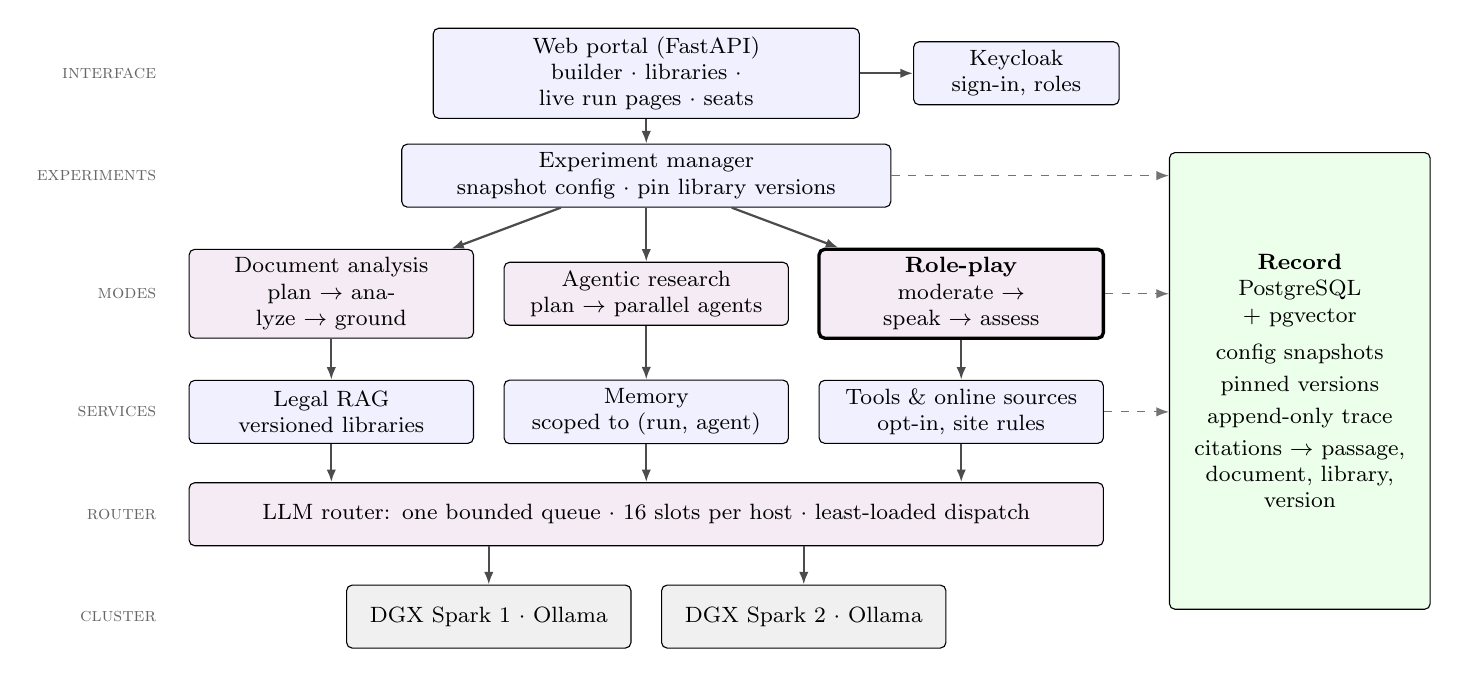
\begin{tikzpicture}[
  font=\footnotesize,
  box/.style={draw, rounded corners=2pt, align=center, minimum height=8mm, inner sep=3pt, fill=#1},
  box/.default={blue!6},
  col/.style={text width=34mm},
  tier/.style={font=\scriptsize\scshape, text=black!60, anchor=east},
  arr/.style={-{Latex[length=1.6mm]}, thick, black!70},
  dsh/.style={-{Latex[length=1.6mm]}, dashed, black!55}
]
% columns at x = -4, 0, 4; rows at y = 0, -1.3, -2.8, -4.3, -5.6, -6.9
\node[box, text width=52mm] (portal) at (0,0) {Web portal (FastAPI) \\ builder $\cdot$ libraries $\cdot$ live run pages $\cdot$ seats};
\node[box, text width=24mm] (kc) at (4.7,0) {Keycloak \\ sign-in, roles};
\node[box, text width=60mm] (mgr) at (0,-1.3) {Experiment manager \\ snapshot config $\cdot$ pin library versions};
\node[box=violet!8, col] (da) at (-4,-2.8) {Document analysis \\ plan $\to$ analyze $\to$ ground};
\node[box=violet!8, col] (aw) at (0,-2.8) {Agentic research \\ plan $\to$ parallel agents};
\node[box=violet!8, col, very thick] (rp) at (4,-2.8) {\textbf{Role-play} \\ moderate $\to$ speak $\to$ assess};
\node[box, col] (rag) at (-4,-4.3) {Legal RAG \\ versioned libraries};
\node[box, col] (mem) at (0,-4.3) {Memory \\ scoped to (run, agent)};
\node[box, col] (tools) at (4,-4.3) {Tools \& online sources \\ opt-in, site rules};
\node[box=violet!8, text width=114mm] (router) at (0,-5.6) {LLM router: one bounded queue $\cdot$ 16 slots per host $\cdot$ least-loaded dispatch};
\node[box=black!6, col] (s3) at (-2,-6.9) {DGX Spark 1 $\cdot$ Ollama};
\node[box=black!6, col] (s4) at (2,-6.9) {DGX Spark 2 $\cdot$ Ollama};
\node[box=green!8, text width=31mm, minimum height=58mm, anchor=north] (rec) at (8.3,-1.0) {\textbf{Record} \\ PostgreSQL + pgvector \\[4pt] config snapshots \\[2pt] pinned versions \\[2pt] append-only trace \\[2pt] citations $\to$ passage, \\ document, library, \\ version};
\draw[arr] (portal) -- (mgr);
\draw[arr] (portal) -- (kc);
\draw[arr] (mgr) -- (da); \draw[arr] (mgr) -- (aw); \draw[arr] (mgr) -- (rp);
\draw[arr] (da) -- (rag); \draw[arr] (aw) -- (mem); \draw[arr] (rp) -- (tools);
\draw[arr] (rag) -- (rag |- router.north); \draw[arr] (mem) -- (router); \draw[arr] (tools) -- (tools |- router.north);
\draw[arr] (router.south -| s3) -- (s3); \draw[arr] (router.south -| s4) -- (s4);
\draw[dsh] (mgr.east) -- (rec.west |- mgr.east);
\draw[dsh] (rp.east) -- (rec.west |- rp.east);
\draw[dsh] (tools.east) -- (rec.west |- tools.east);
\node[tier] at (-6.1,0) {interface};
\node[tier] at (-6.1,-1.3) {experiments};
\node[tier] at (-6.1,-2.8) {modes};
\node[tier] at (-6.1,-4.3) {services};
\node[tier] at (-6.1,-5.6) {router};
\node[tier] at (-6.1,-6.9) {cluster};
\end{tikzpicture}}
\caption{Architecture of the \lab. Rows are tiers in the order a launched run passes through them. Three experiment modes share one set of services, and every model call passes through a single admission point. Everything above the cluster writes to an append-only record (dashed). Inference never leaves university hardware.}
\Description{A tiered block diagram: web portal and sign-in at top; experiment manager; three mode boxes (document analysis, agentic research, role-play); three service boxes (legal retrieval, memory, tools); a single LLM router; two DGX Spark hosts. A tall box on the right labeled Record receives dashed arrows.}
\label{fig:arch}
\end{figure}

Figure~\ref{fig:arch} shows the system. It is a single Python process (FastAPI with asyncio) behind the university's reverse proxy, with sign-in through a self-hosted Keycloak. University accounts are approved automatically; others request access and are approved by an administrator with a viewer, researcher, or administrator role~\cite{gong2026architecture}.

\paragraph{Three modes over shared services.} Each experiment mode is a LangGraph~\cite{langgraph} state graph. \emph{Document analysis} decomposes a question into sub-questions, answers them concurrently from a document or from retrieval, and writes a cited answer. \emph{Agentic research} drafts a research plan that the researcher edits before launch, then runs parallel ReAct-style agents~\cite{yao2023react}, one per sub-question, that search the lab's libraries and, only if the researcher grants the permission for that run, public legal databases and the open web; every page read is first saved into a library, and a page is read only if its site permits AI agents under robots.txt, \texttt{noai} markings, and TDM reservations~\cite{rfc9309,tdmrep,eudsm2019,gong2026network}. \emph{Role-play}, the subject of this paper, is described in Sections~\ref{sec:boundaries}--\ref{sec:provenance}. The three modes share retrieval, memory, tools, the router, and the tracer; they differ in their nodes, not in what they stand on.

\paragraph{Local inference and a single queue.} Two NVIDIA DGX Spark units serve models through Ollama~\cite{ollama}. The lab's model for role-play and document analysis is \code{gemma4}, the E4B size of Google's Gemma~4 family~\cite{gemma4report,gemma4card}: 8 billion parameters including per-layer embeddings (4.5 billion effective), quantized to 4 bits, with a 128K-token context, native function calling, a configurable reasoning (``thinking'') mode, and image and audio input, released under the Apache~2.0 license. Google reports scores for the instruction-tuned E4B of 69.4\% on MMLU-Pro, 58.6\% on GPQA Diamond, and 42.2\% on the $\tau^2$ agentic tool-use benchmark~\cite{gemma4card}. In the lab's own use it has proven capable of what the architecture asks of a model: it returns the moderator's and ledgers' schema-constrained JSON reliably (no unparseable decision or ledger in the 24-turn mediation of Section~\ref{sec:use}~\cite{gong2026moderation}), calls the search tools natively, holds a long transcript within its context, and completed all 1{,}138 model calls of the role-play runs reported here without error. Embeddings for retrieval come from a separate model (\code{nomic-embed-text}). The same hosts serve other open-weight models that a role can be assigned, among them Qwen~3.6 and Hermes~3. In the current configuration no prompt or document is sent to a commercial model API, which matters for a platform whose terms forbid client confidences and student records but whose users will nonetheless upload realistic case material. Benchmarking showed that aggregate throughput plateaus at about 16 concurrent requests per host (160 tokens/s) while 50 concurrent requests still complete, with median latency growing from 1.9\,s to 5.2\,s. Past the plateau, extra requests merely queue inside the inference server. The router therefore admits at most 16 requests per host through one global semaphore and queues the rest itself, recording queue wait separately from model time; otherwise a run that was waiting would be indistinguishable from a run whose model was slow, and timing comparisons across runs would be meaningless.

\paragraph{Reproducibility by construction.} Launching a run copies the experiment's configuration into an immutable snapshot and pins every library it may search---shared libraries and each agent's case files---to a recorded version. Documents are never edited in place; removal and re-reading create new rows, so any recorded version can be searched exactly as it was, and a run page offers ``run again with these versions.'' The trace is append-only: one row per model call, tool call, retrieval, and node transition, with the model's reasoning in its own column.

\paragraph{Designed for lawyers.} Configuration is written by law faculty and students, not programmers. Agents and whole experiments are plain Markdown files with headings such as \emph{Role}, \emph{Objective}, \emph{Bottom line}, \emph{Confidential information}, and \emph{Case files}; headings match by common synonyms (``Walk-away point''), unknown sections are preserved and reported, never dropped. A cast can also be drafted by the model from a news story, court page, or opinion. Because a draft invents bottom lines and confidential facts, real people and private organizations in the source are replaced with invented names before the model sees it and the same substitution is applied to its output: in an early test on a news story about a gravel-pit dispute, instructing the model to invent names was not enough, and it attached an invented secret to the real mining company. Attributing fabricated confidential facts to real private parties is the legal risk worth engineering against; courts, agencies, and places keep their real names.

%% ===================================================================
\section{Information Boundaries in Role-Play}
\label{sec:boundaries}

A role-play is a cycle over a shared public transcript: a moderator judges the latest turn and selects the next speaker; the speaker updates private notes, optionally searches its sources, and speaks; the cycle repeats until the scene ends, and an assessor evaluates the whole. Each participant is specified by a role and objective, optional background, demeanor, tendencies, and priorities, and two private fields: a \emph{bottom line} and \emph{confidential facts}. Table~\ref{tab:process} lists the features of the legal process the role-play is built to reproduce and the mechanism that implements each; Table~\ref{tab:visibility} gives the resulting information-flow policy, and the remainder of this section explains how each is enforced.

\begin{table}[t]
\caption{Features of the legal process and the mechanisms that implement them. The features are shared, in different forms, by negotiation, mediation, and adjudication.}
\label{tab:process}
\small
\begin{tabular}{@{}>{\raggedright\arraybackslash}p{0.19\linewidth}>{\raggedright\arraybackslash}p{0.33\linewidth}>{\raggedright\arraybackslash}p{0.41\linewidth}@{}}
\toprule
Feature & In practice & Mechanism (section) \\
\midrule
Party presentation & Each side develops and argues its own case & A separate agent per party with its own role, objective, and private negotiation ledger (\ref{sec:memory}) \\
Client confidences & Each side holds information the other does not & Bottom line and confidential facts visible only to their owner; memory scoped to (run, agent) (\ref{sec:memory}) \\
Party-controlled disclosure & A side chooses what to put forward and cannot argue from what it withholds & Private case files; a cited passage becomes an exhibit (\ref{sec:exhibits}) \\
Opportunity to respond & The other side can examine and answer what is put forward & Exhibits visible to all from disclosure on; turn rules guarantee each party the floor (\ref{sec:exhibits}, \ref{sec:moderation}) \\
A neutral with limited knowledge & The mediator or judge does not know the parties' private limits & Moderator never sees bottom lines; structured judgments, coded rules (\ref{sec:moderation}) \\
Orderly procedure & Rules govern who speaks, when, and when it ends & Questions answered first, speaking-time balance, intervention cool-down, ending floor (\ref{sec:moderation}) \\
Equal footing & Participants proceed under the same rules and information & Seat parity for human participants (\ref{sec:seats}) \\
A record & What was said and relied on is preserved & Append-only trace, attributed exhibits, citations traced to pinned library versions (\ref{sec:provenance}) \\
\bottomrule
\end{tabular}
\end{table}

\begin{table}[t]
\caption{Information-flow policy of the role-play. ``Own'' means each participant sees only its own. Every row is enforced by what code places in each prompt, not by instructing a model to ignore what it was shown.}
\label{tab:visibility}
\small
\begin{tabular}{@{}p{0.36\linewidth}cccc@{}}
\toprule
Information & Speaker & Other parties & Moderator & Assessor \\
\midrule
Scenario; public transcript & yes & yes & recent window & yes \\
Names, roles, objectives & all & all & all & names \\
Background, demeanor, tendencies & own & own & no & no \\
Bottom line, confidential facts & own & own & no & all \\
Private negotiation ledger & own & own & no & no \\
Case-file passages (uncited) & own & own & no & all \\
Exhibits (all cited passages) & all & all & no & all \\
Moderator's private note & if addressed & no & writes it & no \\
\bottomrule
\end{tabular}
\end{table}

\subsection{Scoped memory and private ledgers}
\label{sec:memory}

Each agent's memory is keyed by \code{(run\_id, agent\_id)}. A two-tier store keeps a verbatim buffer within a token budget and compacts overflow into model-written summaries, embedded and recalled by similarity (pgvector with HNSW indexing~\cite{pgvector}). The scoping is the point: a shared buffer, the default in many agent frameworks, would place one side's private reasoning into the other's context and silently invalidate the exercise. The agent's own reasoning tokens are stored in the trace for researchers but never re-enter any prompt.

Before speaking, an agent updates a \emph{private negotiation ledger} with seven fields: concessions made, concessions received, where things stand, its read on the others, open issues, arguments already made, and next move. The update is a schema-constrained call with reasoning disabled that carries the previous ledger forward; a malformed update keeps the previous one. The ledger serves as work product in the legal sense---the advocate's own analysis, never shown to the other side---and as a correction for two documented failures: re-proposing the same deal~\cite{abdelnabi2023negotiation} and near-universal impasse, which an agent-authored ledger of concessions and open issues has been found to reduce~\cite{andric2026diversity}. The reply prompt ends with a short character reminder restating identity, objective, bottom line, and demeanor, because adherence to initial instructions decays over long dialogs~\cite{li2024instability}.

\subsection{Case files and disclosure by citation}
\label{sec:exhibits}

Real disputes are not argued from a shared library. Each side holds documents the other has not seen and decides which to put in the record. The platform models this with \emph{case files}: libraries attached to one agent and searchable only on that agent's turns, alongside the shared libraries every party may search. Rather than having passages pushed into its prompt, a speaker is given tools---\code{search\_legal\_sources} and \code{search\_case\_file}---and looks things up when it needs to, up to four searches a turn. Passages found are numbered \mk{S1}, \mk{S2} in the order found, those from a case file are marked as unseen by anyone else, and the speaker is told to cite only what a passage says.

The rule is deliberately simple: \emph{every passage a speaker cites enters the record as an exhibit} (Algorithm~\ref{alg:disclose}). After a turn is spoken, code parses the turn for markers, and each cited passage not already on the record is appended to the run's exhibit list as \mk{E1}, \mk{E2}, \ldots, with the speaker and the turn. For a passage from the shared libraries this puts an authority formally on the record; for a passage from the speaker's own case file it is also the passage's disclosure, since no one else could see it before. From then on every participant sees the exhibit and may cite it to rely on it or to answer it, and a later search that returns the same passage reports it as already on the record. An uncited case-file passage never reaches another agent's prompt. The assessor sees all case files and exhibits, so it can judge both what was disclosed and what was withheld.

\begin{algorithm}[t]
\caption{Recording a turn's citations and disclosures (simplified).}
\label{alg:disclose}
\small
\begin{algorithmic}[1]
\Require turn text $t$ by speaker $a$ at turn $k$; passages $F = [f_1..f_m]$ found by $a$ this turn; exhibit list $X$
\For{each marker \mk{S$i$} in $t$}
  \If{$1 \le i \le m$} \Comment{names a passage $a$ actually retrieved}
    \State record citation $\to$ ($f_i$.chunk, document, library, pinned version), verdict \emph{grounded}
    \If{$f_i \notin X$} \Comment{shared or from $a$'s case file}
      \State append $f_i$ to $X$ as \mk{E$|X|$} with speaker $a$, turn $k$ \Comment{now visible to all}
    \EndIf
  \Else
    \State record citation with verdict \emph{unsupported} \Comment{kept, never dropped}
  \EndIf
\EndFor
\For{each marker \mk{E$j$} in $t$}
  \State \textbf{if} $1 \le j \le |X|$ \textbf{then} record as grounded to exhibit $X_j$ \textbf{else} record as unsupported
\EndFor
\end{algorithmic}
\end{algorithm}

Two properties of this rule matter legally. First, disclosure is tied to \emph{reliance}: an agent cannot use a document's content against the other side without putting the document where the other side can read and rebut it, which is the core of the adversarial norm that a party may not argue from evidence it withholds. Second, disclosure is \emph{irreversible and attributed}, as in practice: once in the record, an exhibit cannot be withdrawn, and the run stores who disclosed it and when. The rule is coarser than real procedure---there is no discovery obligation, no privilege log, no objection---and Section~\ref{sec:discussion} discusses what that omits.

\subsection{Seats with parity for human participants}
\label{sec:seats}

Any role may be \emph{played by a person}, chosen per run from the lab's members, so a student can negotiate against AI counterparts or an instructor can play the mediator. The run opens a seat: on their own page the person fills in their profile, signals readiness, and types turns, with a search box over exactly the sources an AI agent in that seat could search. The graph waits for them up to a time limit set at launch.

The governing rule is \emph{seat parity}: a person sees only what an AI in their seat would see---the scenario, their own profile, what is said aloud, and the exhibits. While the run is live, the experiment page, its other runs, and the trace (which contain the other side's bottom line and ledger) redirect the person back to their seat; the full record opens only when the run ends. The seat endpoints verify that the seat belongs to the requesting account, so a person with a view-only account can play without being able to read anything else. Parity makes human and AI turns comparable as data, and in teaching it prevents the obvious shortcut of reading the opponent's instructions.

\subsection{Moderation: structured judgment, coded rules}
\label{sec:moderation}

The moderator is where the principle is most visible. Before each turn after the first, the model answers four questions in a fixed JSON schema at temperature 0 with reasoning disabled: did the last speaker put a direct question to a specific participant; are the parties restating positions without a new proposal, concession, or question; have they clearly agreed or clearly walked away; and who should speak next. Identifiers are constrained to the cast, so nothing is parsed from free text. Code then decides~\cite{gong2026moderation}: the previous speaker is ineligible; a participant asked a direct question answers next, following adjacency-pair ordering~\cite{sacks1974turntaking,nonomura2025whospeaks}; otherwise the model's suggestion stands unless it would put that participant two or more turns ahead of the quietest eligible participant. A reported stall triggers an intervention, at most once per $\max(4, 2n)$ turns for $n$ participants, rotating through reframing, narrowing, and reality testing~\cite{fisher2011yes,johnsen2026mediation}. A scene may end on reported agreement or walk-away only after every participant has spoken twice, because multi-agent exchanges drift toward premature consensus~\cite{yao2025peacemaker,wynn2025talk}; a conclusion reported earlier is logged and ignored. The moderator never sees bottom lines (Table~\ref{tab:visibility}); a moderator that did could steer the parties toward their zone of agreement, which a real mediator cannot do without caucusing.

\subsection{One model by default, a model per role by design}

By default every role, the moderator, and the assessor are played by \code{gemma4}, and every substantive run reported in Section~\ref{sec:use} used it throughout. The architecture nonetheless lets each role name the model that plays it, so that a later study can set one model against another, or swap the assignment between runs to test whether an outcome follows the side or the model. Models without a reasoning mode are called with it off, and a model that writes a tool call as text is read as calling the tool. The motivation is methodological---outcome differences can be attributed to a model rather than a side---and it lets the same scenario be run with different models, local or, once subscription access is enabled, commercial models billed per token, without changing the scenario or the boundaries.

%% ===================================================================
\section{Provenance: From Transcript to Record}
\label{sec:provenance}

A transcript becomes a research record only if each claim in it can be traced to what the speaker was shown. The platform uses three citation namespaces with one resolution rule. In document analysis, markers \mk{1}, \mk{2} index the passages of one retrieval. In agentic research, a run-wide ledger numbers each passage once whichever agent found it, so \mk{3} in the final answer names one passage. In role-play, \mk{S$i$} indexes the passages the speaker found \emph{in that turn}, and \mk{E$j$} indexes the run's exhibits. Each marker becomes a row holding the chunk, document, library, library version, and location (``Turn 7 $\cdot$ Dana Reyes''). A marker that names no passage the model was given is stored with the verdict \emph{unsupported} rather than silently dropped; catching fabrication is the purpose. The run page links each marker to its passage and lists References in citation form with the library version each document was found in.

Turn-scoping of \mk{S$i$} is a deliberate choice. Because passages are numbered afresh each turn, a marker that appears in a turn whose speaker made no search cannot resolve to anything, however plausible it looks and however many times it appeared earlier in the transcript. Repetition across turns lends a marker no legitimacy.

The verification is \emph{referential}, not semantic: it establishes that a cited passage exists, was retrieved by this speaker, and is identified by document and version, not that the passage supports the sentence it is attached to. In evidentiary terms it is closer to authentication---evidence sufficient to support a finding that the item is what its proponent claims~\cite{fre901}---than to a judgment of weight. Semantic support is left to the assessor and to human review.

\subsection{What is enforced and what is recorded}
\label{sec:enforce}

The mechanisms above act at different times, and the distinction is easy to blur. Table~\ref{tab:enforce} separates them. Information flow is \emph{enforced}: each prompt is assembled by code from only the material its recipient may see, so a private fact or uncited case-file passage cannot reach another party however the models behave. Turn order and scene length are enforced the same way. Citation verification, by contrast, is \emph{recorded}: after each turn the verifier resolves every marker and stores a verdict, but the turn enters the public transcript exactly as written, and the verdict is not shown to the speaker, the other parties, the moderator, or the assessor. The run page and PDF report show it to researchers afterward. This was a deliberate first step---recording leaves the behavior under study undisturbed---but it means the platform currently detects fabricated citations without stopping them. Confidential disclosures in speech and concessions past a bottom line are neither enforced nor computed; they are judged only by the assessor.

\begin{table}[t]
\caption{When each property is acted on. \emph{Enforced}: decided by code before or during a turn, so model behavior cannot violate it. \emph{Recorded}: computed by code after a turn and stored for review, with no effect on the run. \emph{Judged}: assessed only by the model-based assessor after the scene.}
\label{tab:enforce}
\small
\begin{tabular}{@{}>{\raggedright\arraybackslash}p{0.52\linewidth}>{\raggedright\arraybackslash}p{0.4\linewidth}@{}}
\toprule
Property & Status \\
\midrule
Private briefs, ledgers, memory, reasoning stay with their owner & Enforced (prompt assembly) \\
Uncited case-file passages stay private; cited ones become exhibits & Enforced (after each turn) \\
A person in a seat sees only what an AI in that seat would & Enforced (server checks) \\
Moderator never sees bottom lines or confidential facts & Enforced (prompt assembly) \\
Turn order, balance, intervention cool-down, ending floor & Enforced (policy code) \\
Run configuration and library versions fixed at launch & Enforced (snapshot, pinning) \\
Each citation names a passage the speaker retrieved & Recorded (verdict per marker) \\
Turn length within the word limit & Recorded (trace note) \\
Confidential facts not revealed in speech; no concession past bottom line & Judged (assessor only) \\
Cited passage supports the claim; legal propositions accurate & Judged (assessor, human review) \\
\bottomrule
\end{tabular}
\end{table}

%% ===================================================================
\section{The Platform in Use}
\label{sec:use}

The platform has been in use since July 2026 by law and computing faculty at the University of Wyoming. This section illustrates the architecture with runs from that period. It is not an evaluation: most runs are development runs, nearly all used one model, and we draw no conclusions about model behavior from them.

\subsection{Usage to date}

Between July 23 and October 20, 2026, the platform completed 35 role-play runs. Twelve were substantive exercises over nine scenarios: an evidentiary hearing on a motion to suppress, run three times (Section~\ref{sec:hearing}); a patent-law debate; a three-party mediation over state trust-land gravel leases, drafted from a news report of Wyoming Supreme Court arguments; a four-party family-law relocation settlement conference; a copyright class-action mediation over generative-AI training; a commercial settlement over losses caused by an autonomous dispatch agent; and a groundwater-depletion dispute staged three ways---under Western water-rights framing, under Buddhist-jurisprudence framing, and the latter again with a library of Buddhist texts as each party's case file. The other 23 were development runs exercising specific mechanisms as they were built: case files and exhibits, human seats, and mixed-model casts. Table~\ref{tab:corpus} summarizes them. Every role in every substantive run, and in all but two development runs, was played by \code{gemma4}; the two exceptions tested the per-role model option with one seat assigned to another locally installed model. The comparative-jurisprudence scenario illustrates a research use the architecture was designed for: the same dispute, parties, and private instructions, varied in one respect, with every other condition fixed by the configuration snapshot.

\begin{table}[t]
\caption{Role-play runs completed July 23 -- October 20, 2026. Model time excludes queue wait; no substantive run waited in the router's queue.}
\label{tab:corpus}
\small
\begin{tabular}{@{}lrr@{}}
\toprule
 & Substantive & Development \\
\midrule
Runs & 12 & 23 \\
Turns (total; longest run) & 286; 100 & 97; 9 \\
Wall-clock minutes (total) & 168 & 50 \\
Model calls; errors & 864; 0 & 274; 0 \\
Prompt / output tokens & 3.44M / 406K & 234K / 130K \\
Runs with exhibits on the record (exhibits) & 3 (5) & 10 (11) \\
Runs with a human seat; with a mixed-model cast & 0; 0 & 2; 2 \\
\bottomrule
\end{tabular}
\end{table}

\subsection{Worked example: case files and exhibits}

A four-turn development run shows the disclosure rule of Section~\ref{sec:exhibits} end to end. Counsel for a service provider and counsel for its client negotiate a termination-for-convenience clause. Each holds a private case file of synthetic test material: the provider's counsel a set of notes on contract law, the client's counsel a model regulation on termination notice. Neither can search the other's.

In turn 1, the provider's counsel searched her case file, cited a passage from the contract-law notes, and so disclosed it; it entered the record as \mk{E1}, attributed to her. In turn 2, the client's counsel searched his case file and cited the model regulation, which became \mk{E2}. In turn 3, the provider's counsel answered the exhibit she had not been able to see until it was cited: ``The Model Regulation \mk{E2} is merely advisory, not controlling law when dealing with sophisticated commercial parties like ours.'' The run stores both exhibits with discloser, turn, document, library, and version; the run page links each marker to its passage; and the assessor received both case files and the exhibit list, so it could judge what each side disclosed and what it held back. This is the behavior the rule is meant to produce: a document enters the exchange when a party relies on it, and from then on the other side can read it and argue against it.

\subsection{Worked example: an evidentiary hearing}
\label{sec:hearing}

To exercise the third setting we staged a hearing on a motion to suppress in a fictional federal prosecution, \emph{United States v.\ Harmon}. Police arrested the defendant after a controlled drug buy, obtained his phone's passcode, and read his text messages without a warrant; a warrant was signed the next morning. The cast was a presiding district judge, defense counsel moving to suppress, and an Assistant U.S.\ Attorney opposing on consent, exigency, and inevitable discovery. The configuration separated law from evidence, as a real hearing does. The controlling authorities---\emph{Riley v.\ California}~\cite{riley2014} and the majority opinion in \emph{Nix v.\ Williams}~\cite{nix1984}, ingested through the CourtListener interface---formed a library all three participants could search. Each side's evidence was a private case file of fictional documents written for the exercise: for the defense, an investigator's memorandum on the arresting officer's body-camera footage; for the government, the officer's incident report. Each counsel also had a bottom line and a confidential fact. We ran the experiment three times, concurrently, at up to 14 turns of 350 words; each run took 9--11 minutes, with no errors and no queue wait.

The mechanisms carried over without change. In every run the judge opened the hearing and questioned both counsel, and the turn rules gave each side the floor. Authorities entered the record through citation: in one run the judge searched the shared library and cited two passages from \emph{Riley} in her opening, which became \mk{E1} and \mk{E2}, and both counsel then argued from those exhibits; in the others, defense counsel put passages of \emph{Riley} or \emph{Nix} on the record. Across the three runs, 18 of 19 citation markers resolved to retrieved passages, and the verifier recorded the remaining one, in which the government's counsel repeated a marker from the defense's turn without having searched, as unsupported.

The information boundaries also held where it mattered for the judge. Neither counsel searched its own case file, so the body-camera memorandum and the incident report never entered the record. The judge, who could not see the case files, repeatedly told counsel that ``neither counsel has yet produced a single exhibit or piece of testimony'' on the scope of the officer's search, and declined to rule on facts not in the record. That is the behavior the architecture is meant to produce: the neutral knows only what the parties put before it.

The runs also showed what the hearing setting needs that the negotiation setting does not. The moderator's impasse interventions are mediation techniques, and three of the six were addressed to the judge (``Judge Eleanor Marsh, pick the single open issue closest to agreement''). The ending rule recognizes agreement or a walk-away but not a ruling, so all three runs ended at the turn limit without a ruling from the bench. And the assessment asks whether the parties reached agreement, which is the wrong question for an adjudication. Section~\ref{sec:discussion} describes the change this calls for.

\subsection{Moderation in a three-party mediation}

The gravel-lease mediation (24 turns, 12 minutes, up to 1{,}000 words a turn) shows the moderation rules operating as specified~\cite{gong2026moderation}. Sixteen turns were assigned by answering a direct question, five by the moderator's choice, and two by the balance rule; all three intervention techniques fired in rotation with the cool-down respected; a conclusion reported after turn 13 was held back because not every participant had yet spoken twice; and the scene ended when the operator's representative withdrew. The run also showed two refinements needed in the rules themselves: because question routing precedes the balance rule, the participant to whom most questions were addressed took 11 of 24 turns; and interventions addressed to whoever speaks next can reach the neutral mediator. Because the rules are code, each is a change to policy that can be tested offline, which would not be true of behavior requested in a prompt.

\subsection{Cost}

Each AI turn costs three model calls: private notes, reply, and moderator. In the gravel-lease run these averaged 3.7\,s, 17.0\,s, and 2.4\,s, and the final assessment 35\,s. The 100-turn family-law conference with four parties took 51 minutes, 43 of them inside the model. Because the router records queue wait separately from model time, these figures can be read as model time. On the current hardware a 100-turn scene at 1{,}000 words a turn takes about an hour, which makes overnight batches of tens of runs per scenario practical.

%% ===================================================================
\section{Discussion}
\label{sec:discussion}

\paragraph{Legal analogues and their limits.}
The information-flow policy borrows from legal practice but simplifies it. Disclosure by citation captures the norm that one may not argue from withheld evidence, but omits discovery obligations, privilege, and objection; a party here may simply never cite an unfavorable document, which is lawful in negotiation but not in litigation. Mediator blindness to bottom lines models a joint session but not a caucus, in which a real mediator learns each side's position in confidence; adding caucus would require a third visibility class (seen by the moderator, not by the other party), which the policy table accommodates. The platform also inverts one legal norm deliberately. Mediation communications are privileged and compromise offers inadmissible~\cite{uma2001,fre408}, to encourage candor; the platform records everything, because a research record that omitted the negotiation would be useless. Participants in human seats are therefore told, in the terms of use, that their turns are logged: the simulation is not a confidential setting even though it simulates one.

\paragraph{Procedure profiles.}
The hearing runs show that the information boundaries and the record generalize across settings, but that orchestration does not: who intervenes, how, and what ends a scene differ by procedure. We therefore plan to make the procedure a first-class part of an experiment's configuration. A \emph{negotiation} profile keeps the current rules. A \emph{mediation} profile directs interventions only to parties, never to the neutral, and adds a caucus, in which the mediator hears one party in confidence (a third visibility class). A \emph{hearing} profile gives the presiding judge control of the floor and of when argument closes, ends the scene when the judge rules, replaces the mediation interventions with procedural ones (directing counsel to the record, or to an unanswered question), and assesses the exchange by adjudicative criteria---whether the ruling rests on the record and the cited authorities---rather than by agreement. Each is a change to policy code and prompts, not to the boundaries, which is the separation the architecture was designed to allow.

\paragraph{From recording to enforcement.}
Citation verdicts are currently recorded, not acted on during a run (Table~\ref{tab:enforce}). The next architectural step is to decide what the platform should do when a marker names no retrieved passage, and there are at least three options, each with a legal analogue. The verdicts can be given to the \emph{assessor}, so that its evaluation starts from computed facts; this changes nothing in the exchange. The verdict can be shown to the \emph{speaker} privately before its turn is final, as a colleague would catch a bad citation before filing. Or an unresolved marker can be \emph{annotated in the public transcript} (``\mk{S1}: no source found''), so that the other parties see it, as opposing counsel or a court would flag a citation that cannot be found. Each changes what is being studied: the first leaves the exchange untouched, the second prevents the error, the third makes the platform a referee. We intend to offer all three as run options, since the right choice depends on whether an experiment studies how models argue unaided or under scrutiny; a teaching deployment would likely annotate publicly by default. The same reasoning applies to other properties that can be computed from the record, such as comparing each party's confidential facts against the public transcript to flag candidate disclosures for human review.

\paragraph{Limitations.}
The platform is in an early phase, before production use. The runs described illustrate the mechanisms; they are few, mostly development runs, nearly all with one model, and they support no claims about model behavior. The moderator's question, stall, and conclusion judgments have not been validated against human coders, and its parameters have not been ablated. Citation verification is referential, not semantic. Outcome fidelity---whether simulated settlements resemble real ones---is untested, and diverse-looking simulations are known to produce unrealistic outcome distributions~\cite{andric2026diversity}. The human-seat runs to date were development tests by the first author. The hearing scenario has been run three times with one set of materials; its evidence documents are fictional and short, and no run reached a ruling under the current ending rule.

\paragraph{Evaluation plan.}
As the corpus of runs grows, the architecture supports four lines of evaluation. (1) \emph{Mechanism ablations}: each boundary can be switched off in a controlled way---a shared instead of scoped memory, no private ledger, case files pushed into prompts instead of searched---and the effect measured on disclosure, repetition, and outcome. (2) \emph{Model comparisons}: because each role names its model, the same scenarios can be run across local open-weight models and hosted frontier models, with the boundaries and record held constant. (3) \emph{Validation}: the moderator's judgments and the assessor's findings can be compared with annotations by law faculty, using the record of what each party was shown. (4) \emph{Teaching}: a classroom deployment in which students take seats against AI counterparts, under IRB review, comparing their disclosure behavior with the agents'.

%% ===================================================================
\section{Conclusion}

Multi-agent simulation can give legal education an inexhaustible supply of counterparts and give legal-AI research a controlled instrument for studying advocacy. Both uses depend on reproducing the structure of the legal process: who knows what, how information enters the record, who may speak, and what was relied on. The \lab builds these properties into its architecture rather than asking the model to observe them: per-agent memory and private ledgers, case files that become exhibits only when relied upon, seats with information parity, coded turn rules around bounded model judgments, and a record that ties every citation to a pinned library version and every run to a fixed configuration. These mechanisms do not depend on which model plays a role, which is what makes the platform suitable for the comparative and longitudinal evaluation that comes next.

\begin{acks}
The \lab is supported by the University of Wyoming School of Computing's 2026--2027 Faculty Fellows Program, in collaboration with the UW College of Law and UW Information Technology, and is hosted by the UW Advanced Research Computing Center. The system was implemented, and this paper drafted, with the assistance of Claude (Anthropic); the authors reviewed all content and are responsible for it. Participant names in the runs described are invented.
\end{acks}

\bibliographystyle{ACM-Reference-Format}
\bibliography{references}

\end{document}
